\subsection{\texorpdfstring{The homomorphism \(\operatorname{Tor}_n^{\mathbf{A}}(\mathbf{P},\mathbf{M})\to \operatorname{Hom}_{\mathbf{A}}(\operatorname{Ext}_{\mathbf{A}}^{n}(\mathbf{M},\mathbf{A}),\mathbf{P})\)}{The homomorphism \textbackslash operatorname\{Tor\}\_n\^{}\{\textbackslash mathbf\{A\}\}(\textbackslash mathbf\{P\},\textbackslash mathbf\{M\})\textbackslash to \textbackslash operatorname\{Hom\}\_\{\textbackslash mathbf\{A\}\}(\textbackslash operatorname\{Ext\}\_\{\textbackslash mathbf\{A\}\}\^{}\{n\}(\textbackslash mathbf\{M\},\textbackslash mathbf\{A\}),\textbackslash mathbf\{P\})}}

Let M be a left A-module, P a right A-module, and n an integer \(\geqslant 0\) . The k-bilinear map (X, p.~129)

\[
c _ {\mathrm{P}; \mathrm{M}, \mathrm{A} _ {s}}: \operatorname{Ext} _ {\mathrm{A}} ^ {n} (\mathrm{M}, \mathrm{A}) \times \operatorname{Tor} _ {n} ^ {\mathrm{A}} (\mathrm{P}, \mathrm{M}) \rightarrow \mathrm{P} \otimes_ {\mathrm{A}} \mathrm{A}
\]

corresponds to a k-linear map

\[
\operatorname{Tor} _ {n} ^ {\mathbf {A}} (\mathrm{P}, \mathrm{M}) \rightarrow \operatorname{Hom} _ {k} \left(\operatorname{Ext} _ {\mathbf {A}} ^ {n} (\mathrm{M}, \mathrm{A}), \mathrm{P}\right);\tag{2}
\]

Moreover, if one equips Ext \(_{A}^{n}\) (M, A) of the structure of right A-module arising from the bimodule structure of A, the image of (2) consists of A-linear maps, as is verified immediately; one deduces from this a k-homomorphism, said to be canonical

\[
\operatorname{Tor} _ {n} ^ {\mathbf {A}} (\mathrm{P}, \mathrm{M}) \rightarrow \operatorname{Hom} _ {\mathbf {A}} \left(\operatorname{Ext} _ {\mathbf {A}} ^ {n} (\mathrm{M}, \mathrm{A}), \mathrm{P}\right).\tag{3}
\]

PROPOSITION 3. --- a) If \(\mathrm{dp}_{\mathbf{A}}(\mathbf{M}) \leqslant n\) , the canonical homomorphism (3) is injective. b) If \(\mathrm{dp}_{\mathbf{A}}(\mathbf{M}) \leqslant n\) , if A is left noetherian and if M is finitely generated, the canonical homomorphism (3) is bijective.

Let us reason by induction on \(n\) . If \(n = 0\) , M is projective, the homomorphism (3) reduces to the canonical homomorphism \(\mathbf{P} \otimes_{\mathbf{A}} \mathbf{M} \to \operatorname{Hom}_{\mathbf{A}} (\mathbf{M}^{*}, \mathbf{P})\) of II, p.~77, and the proposition follows from loc. cit., corollary. If \(n > 0\) , let

\[
0 \rightarrow \mathbf {N} \rightarrow \mathbf {L} \rightarrow \mathbf {M} \rightarrow 0\tag{4}
\]

be an exact sequence of A-modules where L is free (and finitely generated in case b)); then \(\mathrm{dp}_{\mathbf{A}}(\mathbf{N}) \leqslant n - 1\) (X, p.~135, cor. 2, c)) and N is finitely generated in case b).

Let \(\theta\in\mathrm{Ext}_{\mathbf{A}}^{1}(\mathbf{M},\mathbf{N})\) be the class associated with the exact sequence (4) (X, p.~117, def. 1). Let us denote by

\[
u _ {n}: \operatorname{Ext} _ {\mathbf {A}} ^ {n - 1} (\mathrm{N}, \mathrm{A}) \rightarrow \operatorname{Ext} _ {\mathbf {A}} ^ {n} (\mathrm{M}, \mathrm{A}) \quad v _ {n}: \operatorname{Tor} _ {n} ^ {\mathbf {A}} (\mathrm{P}, \mathrm{M}) \rightarrow \operatorname{Tor} _ {n - 1} ^ {\mathbf {A}} (\mathrm{P}, \mathrm{N})
\]

\[
(\alpha \circ \theta) \circ \beta = \alpha \circ (\theta \circ \beta)
\]

the maps defined by \(u_{n}(\alpha) = \alpha \circ \theta\) and \(v_{n}(\beta) = \theta \circ \beta\) . We have for all \(\alpha\in\mathrm{Ext}_{\mathbf{A}}^{n-1}\left(\mathbf{N},\mathbf{A}\right)\) , \(\beta\in\mathrm{Tor}_{n}^{\mathbf{A}}\left(\mathbf{P},\mathbf{M}\right)\left(\mathbf{X},\text{p. 129, prop. 6}\right)\) , so that the diagram

\[
\begin{array}{c c c} \operatorname{Tor} _ {n} ^ {\mathbf {A}} (\mathrm{P}, \mathrm{M}) & \longrightarrow & \operatorname{Hom} _ {\mathbf {A}} \left(\operatorname{Ext} _ {\mathbf {A}} ^ {n} (\mathrm{M}, \mathrm{A}), \mathrm{P}\right) \\ \Big \downarrow v _ {n} & & \operatorname{Hom} (u _ {n}, 1) \Big \downarrow \\ \operatorname{Tor} _ {n - 1} ^ {\mathbf {A}} (\mathrm{P}, \mathrm{N}) & \longrightarrow & \operatorname{Hom} _ {\mathbf {A}} \left(\operatorname{Ext} _ {\mathbf {A}} ^ {n - 1} (\mathrm{N}, \mathrm{A}), \mathrm{P}\right), \end{array}\tag{5}
\]

where the horizontal arrows are the canonical homomorphisms, is commutative. If n = 1, we thus have a commutative diagram:

\pandocbounded{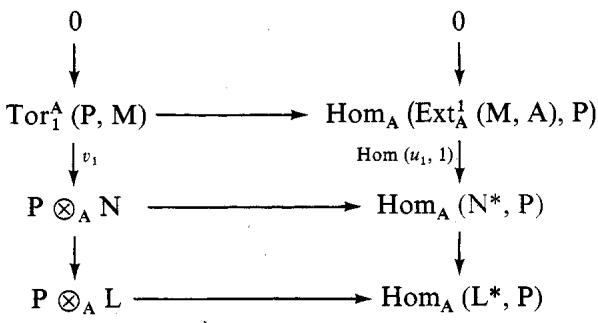
\includegraphics[keepaspectratio]{images/part001_66a54857.jpg}}

where the columns are exact; we deduce the result in this case. If \(n \geqslant 2\) , the maps \(u_n\) and \(v_n\) are bijective (X, p.~128, cor. 4 and p.~131, cor. 3). By the induction hypothesis, the canonical homomorphism

\[
\operatorname{Tor} _ {n - 1} ^ {\mathbf {A}} (\mathrm{P}, \mathrm{N}) \rightarrow \operatorname{Hom} _ {\mathbf {A}} \left(\operatorname{Ext} _ {\mathbf {A}} ^ {n - 1} (\mathrm{N}, \mathrm{A}), \mathrm{P}\right)
\]

is injective (resp. bijective); diagram (5) shows that the same holds for the canonical homomorphism \(\mathrm{Tor}_{n}^{\mathrm{A}}(\mathrm{P},\mathrm{M})\to \mathrm{Hom}_{\mathrm{A}}(\mathrm{Ext}_{\mathrm{A}}^{n}(\mathrm{M},\mathrm{A}),\mathrm{P})\) , which completes the proof.

